% This file was created with tikzplotlib v0.10.1.
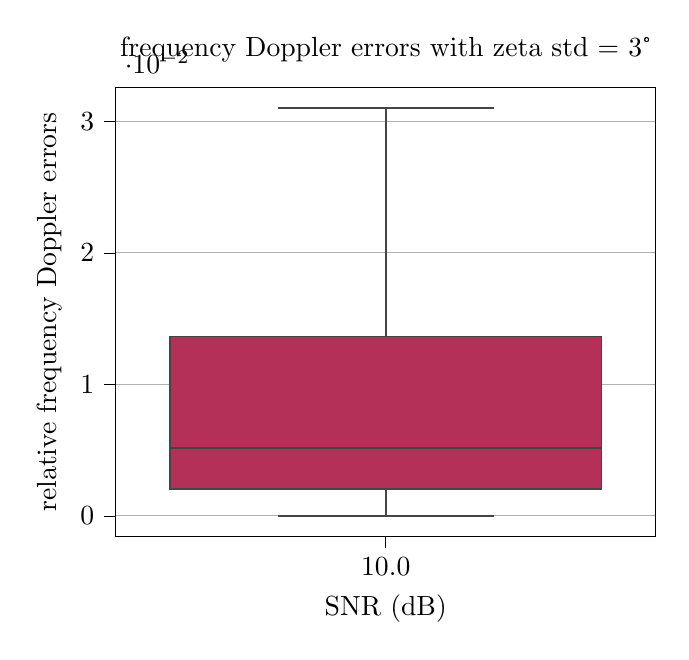
\begin{tikzpicture}

\definecolor{brown1814888}{RGB}{181,48,88}
\definecolor{darkgray176}{RGB}{176,176,176}
\definecolor{darkslategray69}{RGB}{69,69,69}

\begin{axis}[
tick align=outside,
tick pos=left,
title={frequency Doppler errors with zeta std = 3°},
x grid style={darkgray176},
xlabel={SNR (dB)},
xmin=-0.5, xmax=0.5,
xtick style={color=black},
xtick={0},
xticklabels={10.0},
y grid style={darkgray176},
ylabel={relative frequency Doppler errors},
ymajorgrids,
ymin=-0.00155002825977132, ymax=0.0325549152432625,
ytick style={color=black}
]
\path [draw=darkslategray69, fill=brown1814888, semithick]
(axis cs:-0.4,0.00204884150492689)
--(axis cs:0.4,0.00204884150492689)
--(axis cs:0.4,0.0136313524074948)
--(axis cs:-0.4,0.0136313524074948)
--(axis cs:-0.4,0.00204884150492689)
--cycle;
\addplot [semithick, darkslategray69]
table {%
0 0.00204884150492689
0 1.96444912033652e-07
};
\addplot [semithick, darkslategray69]
table {%
0 0.0136313524074948
0 0.0310046905385791
};
\addplot [semithick, darkslategray69]
table {%
-0.2 1.96444912033652e-07
0.2 1.96444912033652e-07
};
\addplot [semithick, darkslategray69]
table {%
-0.2 0.0310046905385791
0.2 0.0310046905385791
};
\addplot [semithick, darkslategray69]
table {%
-0.4 0.00516230868971414
0.4 0.00516230868971414
};
\end{axis}

\end{tikzpicture}
